\documentclass[instructions]{uqthesis}
\hypersetup{hidelinks}
% \usepackage{booktabs}
%\documentclass[final]{uqthesis} 


%*************************************
% FOR YOUR FINAL THESIS
%*************************************

%IMPORTANT! 
%The default document class (above - line 1 & 2) for the template is \documentclass[instructions]{uqthesis} - this document class will show instructional material and examples relevant to the preliminary material in the compiled PDF preview. THESE INSTRUCTIONS ARE FOR YOUR REFERENCE ONLY AND ARE NOT TO BE INCLUDED IN YOUR FINAL THESIS! 

%To turn off these instructions in your final thesis you MUST use the document class \documentclass[final]{uqthesis} 
%To activate the final thesis document class you must UN-COMMENT THIS DOCUMENT CLASS (remove the % from the start of line 2) and comment out the instructional document class on line 1 (add % to the start of line 1). 

%*************************************
% Introduction to template
%*************************************
%This is The University of Queensland Graduate School Official LaTeX Thesis template.

%Be sure to observe the content of comments within the source code, these are prefaced with a percentage symbol.
%Most important instructions have been CAPITALISED.
%To uncomment an inactive command (if required) remove the % from in front of the command.

%Please see the README for more information.

%This file loads the necessary packages, sets the page styles, and defines required macros.
%Edit this if you are comfortable with LaTeX.

%Other tweaks can be made in uqthesis.cls, but change these at your own risk!

%See README for version.

%You must have the memoir class installed.

% ***************************************************
% LaTeX Packages
% ***************************************************
% This file defines the document design.
% Usually it is not necessary to edit this file, but you can use it to change aspects of the design if you want.

%There are essential packages that are contained within the uqthesis.cls which are integral to the template - These must not be deleted.  A list of these packages can be found in the README.tet file

%The packages below are optional, please add or alter as required.

\usepackage{cite}				 %Allows abbreviated numerical citations.
\usepackage{pdfpages}			 %Allows you to include full-page pdfs.
\usepackage{wrapfig}			 %Lets you wrap text around figures.
\usepackage{bm} 				 %Bolded maths characters.
\usepackage{upgreek}			 %Upright Greek characters.
\usepackage{dsfont}				 %Double-struck fonts.
\usepackage{simplewick}			 %For typesetting Wick contractions.
\usepackage{mathtools}		     %Can be used to fine-tune the maths presentation.	
\usepackage{framed}			     %For boxed text.
\usepackage{microtype}			 %pdfLaTeX will fix your kerning.
\usepackage{marvosym}			 %Include symbols (like the Euro symbol, etc.).
\usepackage{color}				 %Nice for scalable pdf graphics using InkScape.
\usepackage{transparent}	     %Nice for scalable pdf graphics using InkScape.
\usepackage{placeins}			 %Lets you put in a \FloatBarrier to stop figures floating past this command.
\usepackage{mdframed,mdwlist}    %Use these for nice lists (less white space).
\usepackage{graphicx}            %Enhanced support for graphics.
\usepackage{float}               %Improved interface for floating objects. 
\usepackage{longtable}           %Allow tables to flow over page boundaries.
\usepackage{mathdots}            %Changed the basic LaTeX and plain TeX commands.
\usepackage{eucal}               %Font shape definitions to use the Euler script symbols in math mode.
\usepackage{array}               %Extending the array and tabular environments.
\usepackage{stmaryrd}            %The StMary’s Road symbol font.
\usepackage{amsthm}              %St Mary Road symbols for theoretical computer science. 
\usepackage{pifont}              %Access to PostScript standard Symbol and Dingbats fonts.
\usepackage{lipsum}              %Easy access to the Lorem Ipsum dummy text.
\usepackage{enumerate}           %Enumerate with redefinable labels. 
\usepackage[all]{xy}             %This is a special package for drawing diagrams.
\usepackage{amsmath}             %ATypesetting theorems (AMS style).
\usepackage{amssymb}             %Provided an extended symbol collection.
\usepackage[utf8]{inputenc}      %Allowed all displayable utf8 characters to be available as input.
\usepackage{fancyhdr}            %Extensive control of page headers and footers.
\usepackage{blindtext}           %Produced 'blind' text for testing.
\usepackage{tikz}                %To create graphic elements.
\usepackage[figuresright]{rotating}	%Allows large tables to be rotated to landscape.
\usepackage{makecell}
\usepackage{tabularx}
\usepackage{titlesec}


\usetikzlibrary{shapes.geometric, arrows}
%You can add more packages here if you need


%This defines some macros that implement Latin abbreviations
%COMMENT OUT OR DELETE IF UNDESIRED.
\newcommand{\via}{\textit{via}} %Italicised via.
\newcommand{\ie}{\textit{i.e.}} %Literally.
\newcommand{\eg}{\textit{e.g.}} %For example.
\newcommand{\etc}{\textit{etc.}} %So on...
\newcommand{\vv}{\textit{vice versa}} %And the other way around.
\newcommand{\viz}{\textit{viz}.} %Resulting in.
\newcommand{\cf}{\textit{cf}.} %See, or 'consistent with'.
\newcommand{\apr}{\textit{a priori}} %Before the fact.
\newcommand{\apo}{\textit{a posteriori}} %After the fact.
\newcommand{\vivo}{\textit{in vivo}} %In the flesh.
\newcommand{\situ}{\textit{in situ}} %On location.
\newcommand{\silico}{\textit{in silico}} %Simulation.
\newcommand{\vitro}{\textit{in vitro}} %In glass.
\newcommand{\vs}{\textit{versus}} %James \vs{} Pete.
\newcommand{\ala}{\textit{\`{a} la}} %In the manner of...
\newcommand{\apriori}{\textit{a priori}} %Before hand.
\newcommand{\etal}{\textit{et al.}} %And others, with correct punctuation.
\newcommand{\naive}{na\"\i{}ve} %Queen Amidala is young and \naive{}.

% ***************************************************
% Title page
% ***************************************************
%***THESIS TITLE***
%Use Sentence Case (capitalise only the first word and proper nouns).
\title{Image Detection with RISC-V Processor on FPGA}
\subtitle{Project Proposal}

%***YOUR NAME***
%Do not include initials or middle names. Do not include your supervisor(s)' name(s).
\author{Joshua Wallace}
\studentnumber{45809978}
%***YOUR CURRENT DEGREES***
%Use abbreviations. Do not include the date or location of your degree. Do not include the degree for which this thesis is being submitted.
\currentdegrees{Project Proposal}

%***ORCID ID***
%Add and hyperlink your ORCID

%***YEAR OF SUBMISSION***
\date{2024}
%***TYPE OF DEGREE***
\submittedfor{Thesis - METR4911}


%***YOUR SCHOOL***
%Use Title Case (capitalise every word which is not a conjunction or preposition).
%See - http://blog.apastyle.org/apastyle/2012/03/title-case-and-sentence-case-capitalization-in-apa-style.html - for help.
\school{School of Information Technology and Electrical Engineering}

\begin{document}

\frontmatter
% Assemble title page
\maketitle
\clearpage

% ***************************************************
% Preface
%****************************************************
% \section{Abstract}
% \normalfont
% %Open abstract.tex to edit
% % ***************************************************
% Abstract
% ***************************************************
% TO PRODUCE A STAND-ALONE PDF OF YOUR ABSTRACT, uncomment this section and the \end{document} at the end of the file by removing the % from the start of each line.

%\documentclass[12pt, a4paper]{memoir}

%% ***************************************************
% LaTeX Packages
% ***************************************************
% This file defines the document design.
% Usually it is not necessary to edit this file, but you can use it to change aspects of the design if you want.

%There are essential packages that are contained within the uqthesis.cls which are integral to the template - These must not be deleted.  A list of these packages can be found in the README.tet file

%The packages below are optional, please add or alter as required.

\usepackage{cite}				 %Allows abbreviated numerical citations.
\usepackage{pdfpages}			 %Allows you to include full-page pdfs.
\usepackage{wrapfig}			 %Lets you wrap text around figures.
\usepackage{bm} 				 %Bolded maths characters.
\usepackage{upgreek}			 %Upright Greek characters.
\usepackage{dsfont}				 %Double-struck fonts.
\usepackage{simplewick}			 %For typesetting Wick contractions.
\usepackage{mathtools}		     %Can be used to fine-tune the maths presentation.	
\usepackage{framed}			     %For boxed text.
\usepackage{microtype}			 %pdfLaTeX will fix your kerning.
\usepackage{marvosym}			 %Include symbols (like the Euro symbol, etc.).
\usepackage{color}				 %Nice for scalable pdf graphics using InkScape.
\usepackage{transparent}	     %Nice for scalable pdf graphics using InkScape.
\usepackage{placeins}			 %Lets you put in a \FloatBarrier to stop figures floating past this command.
\usepackage{mdframed,mdwlist}    %Use these for nice lists (less white space).
\usepackage{graphicx}            %Enhanced support for graphics.
\usepackage{float}               %Improved interface for floating objects. 
\usepackage{longtable}           %Allow tables to flow over page boundaries.
\usepackage{mathdots}            %Changed the basic LaTeX and plain TeX commands.
\usepackage{eucal}               %Font shape definitions to use the Euler script symbols in math mode.
\usepackage{array}               %Extending the array and tabular environments.
\usepackage{stmaryrd}            %The StMary’s Road symbol font.
\usepackage{amsthm}              %St Mary Road symbols for theoretical computer science. 
\usepackage{pifont}              %Access to PostScript standard Symbol and Dingbats fonts.
\usepackage{lipsum}              %Easy access to the Lorem Ipsum dummy text.
\usepackage{enumerate}           %Enumerate with redefinable labels. 
\usepackage[all]{xy}             %This is a special package for drawing diagrams.
\usepackage{amsmath}             %ATypesetting theorems (AMS style).
\usepackage{amssymb}             %Provided an extended symbol collection.
\usepackage[utf8]{inputenc}      %Allowed all displayable utf8 characters to be available as input.
\usepackage{fancyhdr}            %Extensive control of page headers and footers.
\usepackage{blindtext}           %Produced 'blind' text for testing.
\usepackage{tikz}                %To create graphic elements.
\usepackage[figuresright]{rotating}	%Allows large tables to be rotated to landscape.
\usepackage{makecell}
\usepackage{tabularx}
\usepackage{titlesec}


\usetikzlibrary{shapes.geometric, arrows}
%You can add more packages here if you need


%This defines some macros that implement Latin abbreviations
%COMMENT OUT OR DELETE IF UNDESIRED.
\newcommand{\via}{\textit{via}} %Italicised via.
\newcommand{\ie}{\textit{i.e.}} %Literally.
\newcommand{\eg}{\textit{e.g.}} %For example.
\newcommand{\etc}{\textit{etc.}} %So on...
\newcommand{\vv}{\textit{vice versa}} %And the other way around.
\newcommand{\viz}{\textit{viz}.} %Resulting in.
\newcommand{\cf}{\textit{cf}.} %See, or 'consistent with'.
\newcommand{\apr}{\textit{a priori}} %Before the fact.
\newcommand{\apo}{\textit{a posteriori}} %After the fact.
\newcommand{\vivo}{\textit{in vivo}} %In the flesh.
\newcommand{\situ}{\textit{in situ}} %On location.
\newcommand{\silico}{\textit{in silico}} %Simulation.
\newcommand{\vitro}{\textit{in vitro}} %In glass.
\newcommand{\vs}{\textit{versus}} %James \vs{} Pete.
\newcommand{\ala}{\textit{\`{a} la}} %In the manner of...
\newcommand{\apriori}{\textit{a priori}} %Before hand.
\newcommand{\etal}{\textit{et al.}} %And others, with correct punctuation.
\newcommand{\naive}{na\"\i{}ve} %Queen Amidala is young and \naive{}.

%\begin{document}

%\begin{center}
	%\textbf{\large Your title goes here}

	%\textbf{Abstract}

	%Your Name, The University of Queensland, 20??
%\end{center}

This thesis presents an extensible approach for implementing convolution-based image processing algorithms on a RISC-V system on chip. A RISC-V system on chip is interfaced with a Xilinx Artix-7 FPGA using a Wishbone B4 bus interface for hardware acceleration of convolution operations.
The aim of this thesis is to explore the feasibility of implementing hardware acceleration of convolutional neural networks (CNNs) on FPGAs by optimising the convolution layer at hardware for highly resource-constrained devices.

Three architectural approaches for convolution are presented to overcome the resource constraints of FPGAs: a fully parallel implementation achieving maximum throughput but exceeding available resources, a partially folded architecture presenting a tradeoff between throughput and resource utilisation, and a fully folded single-MAC implementation.
The design is validated using an 8x8 pixel grayscale digit dataset with 8-bit precision, representing a storage size of 2040 bytes. 
A pooling layer, activation function and fully connected layer are added to the design to form a complete CNN through generic VHDL modules.
The CNN achieves an 87\% accuracy on the dataset, and is quantized to reduce the bit width from a 32-bit floating point representation to an 8-bit integer representation without loss of accuracy.

The convolution operation is benchmarked as it is the primary bottleneck for latency in a CNN, due to the number of SIMD operations required.
The fully parallel implementation is shown to be impractical for the given FPGA, due to the limited resources available but is capable of completing the operation in a single clock cycle.
The partially folded design provides a 88x reduction in utilisation of the FPGA resources while completing the operation in 49 clock cycles for the given dataset (49x).
A fully folded implementation is suboptimal, as the extra control logic required to manage the dataflow requires significant additional resources which negates the use of a single MAC whilst increasing the latency, with the operation completing in 1960 clock cycles.
Assembling the blocks and connecting it to a RISC-V system on chip is shown to be a feasible approach with folding introduced to enable synthesis.

The partially folded architecture emerged as the optimal solution, demonstrating 46.9x speedup over CPU implementation while requiring minimal FPGA resources.
However, the design is not as performant as a GPU, with a throughput of 204,000 images/s compared to 980,000 images/s for a GPU (P100).
This is not a constraint on the speed of the design, but rather a limitation of the FPGA due to constraints on the number of MAC units that can be implemented.
Quantitative analysis shows the partially folded implementation achieves an efficiency metric of 26,153.8 images/s per percentage LUT utilization, significantly outperforming the fully folded design's 4,159.9 efficiency.
This also surpasses the parallel implementation's 1,159.9 efficiency, due to the large number of MACs required.
The approach is limited by the size of the convolution kernel due to timing constraints, as larger kernels introduce quadratic increases in computational latency.
The produced layers are synthesizable and can be used as a building block for future hardware accelerators on a system on chip.

%\end{document}

% \clearpage
% ***************************************************
% \section*{Declaration by author}
%DO NOT EDIT.
% % ***************************************************
% Declaration by Author
% ***************************************************
% This is the DECLARATION BY AUTHOR
% All candidates to reproduce this section in their thesis verbatim
% DO NOT EDIT!
%
\begin{instructional}
    \textit{(All candidates to reproduce this section in their thesis verbatim)\\}
\end{instructional}

\noindent
This thesis is composed of my original work, and contains no material previously published or written by another person except where due reference has been made in the text. I have clearly stated the contribution by others to jointly-authored works that I have included in my thesis.\\

\noindent
I have clearly stated the contribution of others to my thesis as a whole, including statistical assistance, survey design, data analysis, significant technical procedures, professional editorial advice, financial support and any other original research work used or reported in my thesis. The content of my thesis is the result of work I have carried out since the commencement of my higher degree by research candidature and does not include a substantial part of work that has been submitted to qualify for the award of any other degree or diploma in any university or other tertiary institution. I have clearly stated which parts of my thesis, if any, have been submitted to qualify for another award.\\

\noindent
I acknowledge that an electronic copy of my thesis must be lodged with the University Library and, subject to the policy and procedures of The University of Queensland, the thesis be made available for research and study in accordance with the Copyright Act 1968 unless a period of embargo has been approved by the Dean of the Graduate School. \\

\noindent
I acknowledge that copyright of all material contained in my thesis resides with the copyright holder(s) of that material. Where appropriate I have obtained copyright permission from the copyright holder to reproduce material in this thesis and have sought permission from co-authors for any jointly authored works included in the thesis.

\clearpage
%YOU MUST EDIT THIS DOCUMENT.
% ***************************************************
% PRELIMINARY PAGES
% ***************************************************
% The instructions contained within this part of the thesis template need to be suppressed from the final thesis. There are instructions on how to do this in the MainThesis.tex file.

% To ensure your work is not suppressed with the instructions please add your text only where instructed.


\clearpage
\pagestyle{headings}

\chapter[Table of Abbreviations ]{Table of Abbreviations}

%If the auto-sizing of the tables annoys you, consider the tabularx package.

%List of abbreviations.
\begin{center}
	\small
	\begin{longtable}{ll}
	\toprule
	Abbreviations & {} \\
	\bottomrule
	FPGA			& Field Programmable Gate Array \\
	ASIC			& Application Specific Integrated Circuit \\
	CPU				& Central Processing Unit \\
	GPU				& Graphical Processing Unit \\
	SoC				& System on Chip \\
	ISA				& Instruction Set Architecture \\
    RISC            & Reduced Instruction Set Computer \\
	CISC            & Complex Instruction Set Computer \\
	IO				& Input Output \\
	RTOS			& Real Time Operating System \\
	CNN			    & Convolutional Neural Network \\
    YOLO            & You Only Look Once \\
	VGA				& Video Graphics Array \\
	\hline 
	\end{longtable}
\end{center}

\clearpage

%***Table of Contents***
%These generate the table of contents, list of figures, and list of tables from items tagged with a \label{} command.
\tableofcontents
	\clearpage
\listoffigures
\listoftables

% \input{./PreliminaryAndBackPages/Symbols.tex} %List of symbols. REMOVE IF NOT NEEDED.

%***End of front matter***

% ***************************************************
% Thesis Content
%****************************************************
\mainmatter

%Each chapter is a separate .tex file. Use \input to load them here, as demonstrated below for Chapter 1 and Chapter 2.
%We recommend keeping each in a separate subfolder, with its accompanying figures, etc. This is how the template is currently structured.
%If you wish to divide your thesis into parts (each containing multiple chapters), us the \part{} command.

\chapter[Introduction]{Introduction}
\label{Chap:Intro}

% ***************************************************
% Introduction
% ***************************************************


\section{Motivation}

In recent years, the demand for efficient and versatile image processing systems has surged across various domains, including surveillance, medical imaging, autonomous vehicles, and more. 
Field Programmable Gate Arrays (FPGAs) provide a reconfigurable, low-power embedded platform with parallel processing capabilities akin to graphic processing units (GPUs) commonly used to accelerate demanding computing tasks. 
Image processing is a good candidate for such application of parallel processing, due to the increasing algorithm complexity and large volume of data involved \cite{Efficient}.
These processes have a shared step in the form of convolution, which is a compute-heavy operation often parallelised in software-based implementations.
Hence, FPGAs could provide a suitable platform for real-time image processing tasks, offering a balance of performance, power efficiency, and flexibility.

One significant aspect of image processing systems is the choice of the underlying processor architecture. 
Traditional approaches often rely on general-purpose CPUs or GPUs to execute image processing tasks. 
However, these architectures may not always offer the best balance of performance, power efficiency, and flexibility for image processing applications. 
In recent years, the RISC-V instruction set architecture (ISA) has gained traction as an open, customizable, and energy-efficient alternative to proprietary processor designs.
These soft processors can be implemented on FPGAs, providing a controllable and scalable platform for deferring image processing tasks to dedicated hardware, enabling for parallelisation.

This project will focus on the exploration and implementation of image detection algorithms using the RISC-V processor architecture deployed on an FPGA platform. 
By leveraging the configurability of FPGAs and the energy efficiency of the RISC-V ISA, this research aims to develop a scalable and adaptable solution for handling the core component of image processing tasks using FPGA-accelerated hardware.
The data processing capacity is large that the processing speed must be strict to meet the demands of real-time time image transmission \cite{Video}.
Hence, an FPGA system-on-chip (SoC) offers a means for a low power consumption, low latency but high throughput platform - all of which are essential for the increasing computational demands of image processing tasks \cite{Throughput}.

The work will produce a hardware implementation of an image processing system that can be controlled by a RISC-V processor, and demonstrate the benefits of FPGA-based hardware acceleration for image processing tasks.

\section{Definition}

Traditional software-based image processing techniques on embedded systems lack the parallelisation of larger distributed systems which use GPU architecture to process images.
This project aims to provide a robust and extensible platform for image processing tasks which can be used as a building block for more complex image processing pipelines on an FPGA platform.
By allowing for extensibility of the image processing pipeline, the project aims to provide a flexible platform for future research into the use of FPGAs in the field of image processing.

This projects aims to:
\begin{itemize}
    \item Demonstrate the practicality and benefits of FPGA-based hardware acceleration for image processing tasks.
    \item Illustrate the practicality of neural network layers being applied to resource-limited devices
    \item Demonstrate the control of an image processing pipeline using a RISC-V softcore processor.
    \item Evaluate the performance, efficiency, and scalability of a hardware-implemented image processing system.
\end{itemize}

\section{Scope}

A scope has been defined to better target the aims of this thesis, and exclude any work which is deemed to not be primary to the aims.
The thesis is focused on implementing a convolutional core, and by extension a convolutional neural network, to be used as a hardware accelerator for image processing tasks, and interfaced to with a RISC-V processor.
The scopes of this thesis are hence defined as:

\begin{itemize}
    \item Development of a hardware-implemented convolutional core to accelerate image processing tasks.
    \item Extension of this core to implement a convolutional neural network.
    \item Configuration of neural network layers to be mapped onto the FPGA fabric.
\end{itemize}

There are a number of components which are outside of the scope of this thesis due to the broadness of image processing techniques:
\begin{itemize}
    \item Implementing of image processing techniques which use convolution but extend beyond it
    \item Training of a CNN on FPGA
    \item Finetuning of a CNNs
\end{itemize}
\cleardoublepage
\chapter[Background]{Background}

\label{Chap:Background}

\section{Background}
A review of existing literature relevant to the topic has been conducted to provide a basis for the work. 
The related works to the research were selected zx: Field-Programmable Gate Arrays (FPGAs), RISC-V processors, image detection methods, and convolutional neural networks (CNNs). 
These are broadly discussed below, with a focus on the application of these technologies to image detection and hardware implementations.


\subsection{Image Detection and Analysis}
Image analysis is the process of extracting features from an image, to simplify it into a form that is more easily interpreted \cite{Mathworks}.
This often includes edge detection, object recognition, and image classification as parts of the processing pipeline.
Edge detection forms the basis of many image analysis techniques, as it is used to localize the variations in the image and to identify the physical phenomena which produce them.
These are generally classed as gradient-based or Laplacian based, though gradient-based algorithms are more widely used \cite{Gradient}.

The Robert, Prewitt and Sobel techniques are the most prominent of the gradient-based algorithms, applying kernels to the image to detect edges \cite{Segmentation}.
\cite{XSG, Sobel, Canny, Aerial, Video} all provide a hardware implementation of the these filters, utilising the parallel processing capabilities of FPGAs to accelerate the gradient operations.
These designs realized improved efficiency in performance defined as increased throughput, and resource utilisation. 
Hence, FPGAs can provide a platform for processing real time algorithms on application-specific hardware with substantially higher performance than programmable digital signal processors (DSPs) \cite{RTEdge}.
This strongly indicates that FPGA-based implementations of image detection algorithms can offer significant improvements in running time for a range of digital signal processing methods, but were benchmarked only against microcontroller-based CPU platforms and not parallelised platforms.


The general pipeline for image detection and analysis is shown in Figure \ref{fig:pipeline}. 
This covers the available techniques which can be abstracted into hardware, to provide a high-speed, real-time image detection system.

\begin{figure}[h]
    \centering
    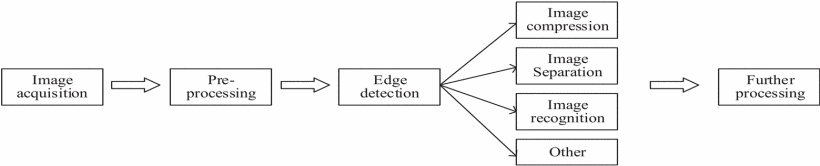
\includegraphics[width=1\textwidth]{Assets/Pipeline.png}
    \caption{Pipeline for image analysis techniques \cite{RTEdge}}
    \label{fig:pipeline}
\end{figure}

\cite{SoCImage, Aerial} follow a similar pipeline to Figure \ref{fig:pipeline}, with the image being captured by a camera module, and then processed by an FPGA though using differing image techniques.
These found that FPGAs can accelerate the required multiplication and addition operators separately - required for classical, and deep learning, based techniques \cite{ResourceEfficient}.


\subsection{Convolutional Neural Networks and Deep Learning}
Convolutional neural networks (CNNs) are a type of artificial neural network that is primarily used for image detection, as it uses the convolution kernel to detect features in the image.
Due to the lack of memory in low-end FPGA models, the CNN is optimal for an image processing task on SoC, as it has a low number of weights and biases relative to other neural networks \cite{Drowsiness}
The convolution operation requires a large number of multiply-accumulate (MAC) operations, and is the primary bottleneck in the performance of CNNs.
The operation must window over the entire image, and the number of MAC operations is proportional to the size of the image and the number of filters in the layer.
Hence, the CNN is computationally intensive, demanding a significant quantity of operations for high accuracy \cite{Linear}.
However, the proceeding \cite{Drowsiness} paper found that the use of an embedded co-processor makes the implementation of CNN less challenging on the FPGA platform, as the network can be designed in a systems language such as C.
This can then be compiled and translated into machine code, as there exists a toolchain for RISC-V.


Similar works for image-analysis using different neural network architectures have also been implemented using FPGA hardware.
\cite{Yolo, SparseYolo} demonstrates a hardware implementation of the You Only Look Once (YOLO) algorithm using a Xilinx Virtex-7 FPGA. 
Like the CNN hardware implementations, the architecture is focused on accelerating the convolution operation - and is a common denominator in the performance neural networks in hardware.
This acceleration is not specific to the convolution operator, and can be applied to any intensive operation in the network as the FPGA has little overhead on each operator when compared to traditional platforms \cite{Overhead}.
This is corroborated by \cite{Throughput}, which found that the implementation of hybrid neural networks on a Xilinix Virtex-7 690T FPGA achieved 4.13 times higher throughput than state of the accelerators in 2019.


\subsection{RISC-V}
Instruction set architectures (ISAs) define the operations a processor can execute, however, the majority of ISAs are proprietary and require licensing to use.
Reduced Instruction Set Computing (RISC) is a form of ISA which offers a simpler, more efficient design than the traditional Complex Instruction Set Computing (CISC) ISAs - such as the prevalent x86 instruction set \cite{Arm}.
Arm and RISC-V are the two most prominent RISC ISAs, with Arm being the most widely used in embedded systems but with RISC-V offering royalty-free licensing and an open-source nature.
The lack of licensing fees and the open-source nature of RISC-V has led to its increasing popularity in the embedded systems domain \cite{Neutron}.
It is estimated that the number of chips utilising RISC-V technology "will grow 73.6 percent per year to 2027, when there will be some 25 billion AI chips produced, accounting for US \$291 billion in revenue" \cite{Drowsiness}.


There exists a number of FPGA implementations to create softcore processors using the RISC-V ISA \cite{RISCFPGA}. 
This 2023 paper \cite{Neutron} demonstrates a RISC-V implementation of the NEORV32 core, using a Wishbone bus interface. 
The authors selected the NEORV32 core due to it being vendor-agnostic and platform independent, with the project being highly documented.
The softcore nature allows for the implementation details to be customised to the specific application, such that the core can be adapted to the specific use case \cite{DCT}. 
The NEORV32 processors offers a system-on-chip (SoC) Harvard architecture, with a 32-bit RISC-V processor, and a range of peripherals.
It supports UART, SPI, standard GPIO and the Wishbone b4 external bus interface for SoC connectivity \cite{NEORV32}.


As it is an open-source ISA, RISC-V has the added benefit of being extensible and modular \cite{Cryptography}, allowing for instructions to be added to the processor.
\cite{Reconfigurable} utilises this to create custom instructions within the RISC-V ISA to accelerate the expensive convolution operation for a CNN.
Other applications have also extended the architecture to include custom instructions for frequently used and computationally-expensive operations.

\subsection{Field-Programmable Gate Arrays}
Field Programmable gate arrays (FPGAs) provide flexible compute resources that can be reconfigured to suit a wide range of applications.
Similar to graphics processing units (GPUs), FPGAs offer parallel processing capabilities, but with the added benefit of reconfigurability \cite{Parallelism}.
The ability to develop custom logic designs is not unique to FPGAs, as application-specific integrated circuits (ASICs) also offer this capability.
ASICs offer better optimization in many aspects than FPGAs, but cannot be reconfigured and require a large upfront cost for design and fabrication \cite{AsicOptimization}.
This makes FPGAs a more suitable platform for low-volume production and prototyping, as they offer a faster development cycle and lower cost than ASICs.

These reconfigurable platforms are optimal for edge applications on images, due to the parallelised pipeline structure, which enables high-speed processing of large amounts of image data, and it's high processing speed ensures real-time image data processing \cite{Video}.
FPGAs in particular have been studied extensively in the field of image detection, as replacements to existing hardware infrastructures due to the increasing complexity of algorithms \cite{ResearchFPGA}.
They offer low latency and low power consumption due to their computing characteristics.
However, the ability to configure oftens mean that resource constraints and utilisation must be considered when designing the system, such as with many embedded devices.


Figure \ref{fig:gradient} shows an implemention of a hardware-accelerated edge-detection algorithm for video images, using the Intel Cyclone IV FPGA platform direct from a camera module. 
This requires a camera module, FPGA and uses a VGA monitor to display the output - but does not use a softcore processor. 

\begin{figure}[h]
    \centering
    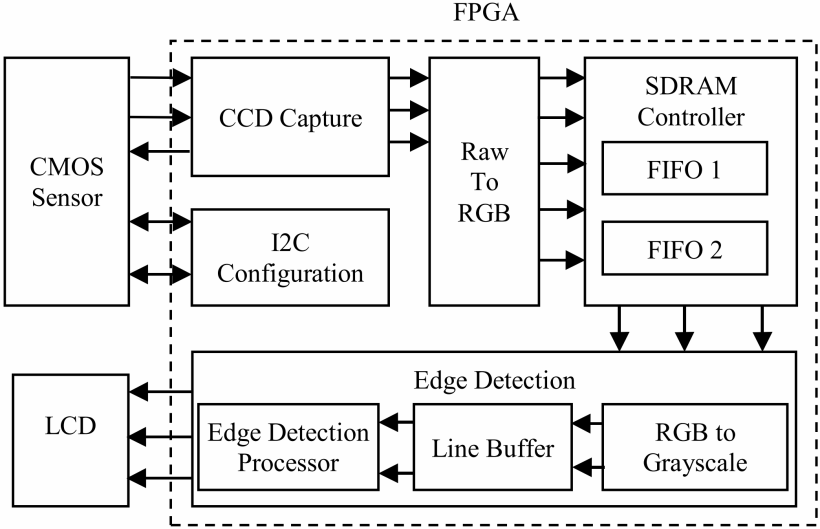
\includegraphics[width=1\textwidth]{Assets/Gradient.png}
    \caption{Video detection FPGA pipeline \cite{Gradient}}
    \label{fig:gradient}
\end{figure}


This pipeline has the core advantage over traditional CPU architectures which are serially structured, as it can perform the operations in hardware and in parallel. 
Hence, an image processing system employing an FPGA as the primary control chip is better suited to the low-latency and high speed demands of real-time image processing \cite{RTEdge}.
Applying a softcore processor to such a pipeline would allow for improved control on a real-time system. 
Furthermore, custom instructions can be added to optimise repeat operations at the systems level whilst maintaining the advantage of performing the processing using the hardware.

\chapter[Topic]{Topic}

\label{Chap:Topic}

\section{Topic}
Image detection, a critical task in computer vision, involves identifying and locating objects within images. 
Traditional software-based approaches for image detection often face challenges related to processing speed and resource utilization, particularly when dealing with large datasets or real-time applications. In response to these challenges, I propose leveraging Field-Programmable Gate Arrays (FPGAs) to accelerate image detection algorithms in hardware. By offloading computationally intensive tasks to FPGA-based hardware accelerators, we aim to significantly enhance the performance and efficiency of image detection systems.

The integration of FPGA-based hardware acceleration offers several compelling advantages. 
Firstly, FPGAs provide inherent parallelism and customizable hardware architectures, enabling efficient execution of image processing algorithms. 
This parallelism can lead to substantial improvements in processing speed, making real-time image detection feasible for applications such as surveillance, autonomous vehicles, and industrial automation. Additionally, FPGA-based solutions offer flexibility and scalability, allowing for the optimization of hardware resources to suit specific image detection requirements. 
Their adaptability is particularly advantageous in scenarios where the detection algorithms need to be customized or updated frequently.

Furthermore, hardware-accelerated image detection using FPGAs can lead to significant reductions in power consumption compared to traditional CPU-based approaches, making it suitable for resource-constrained environments and embedded systems. 
By harnessing the computational efficiency of FPGA-based acceleration, we can achieve higher throughput and lower latency, thereby improving the responsiveness and effectiveness of image detection systems. 
Overall, this research aims to demonstrate the practical significance and utility of FPGA-based hardware acceleration in advancing the capabilities of image detection technology, paving the way for more efficient and scalable solutions in various domains.

\section{Aims}
This projects aim to:
\begin{itemize}
    \item Demonstrate the feasibility and benefits of FPGA-based hardware acceleration for image detection algorithms.
    \item Demonstrate the control of the image detection algorithm using a RISC-V softcore processor.
    \item Evaluate the performance, efficiency, and scalability of a FPGA-based image detection system.
    \item Investigate the potential applications and use cases of FPGAs for image detection tasks in real-world scenarios.
\end{itemize}

It will not include the development of a new image detection algorithm or method, but rather the implementation of existing algorithm(s) for hardware-acceleration, and the control through a RISC-V softcore processor.

\section{Overview}
The work can be divided into subcomponents to provide a timeline and structure to the project, as dependencies on previous work are required to progress.

\subsection{Hardware}
The work will require the Xilinx Artix 7 XC7A100T FPGA, and a corresponding board to access the FPGA resources and I/O ports.
A Digilent Basys 3 board is available initially for development, however, a Digilent Nexys A7-100T board may be required depending on resource limits.
Both these boards use the Artix 7 XC7A100T FPGA, and have VGA output ports to allow for processed images to be displayed to an external monitor.
A camera module will be connected to the FPGA, and the NEORV32 processor will be used to control the image detection algorithm.
This module has currently not been selected in it's entirety, but initial trials will be conducted with an available VGA OV7670 camera module.
The module has been selected due to it's availability, compatability and previous research \cite{SoCImage} conducted with it.

Figure \ref{fig:overview} below provides an overview of the hardware components and their connections.

\begin{figure}[h]
    \centering
    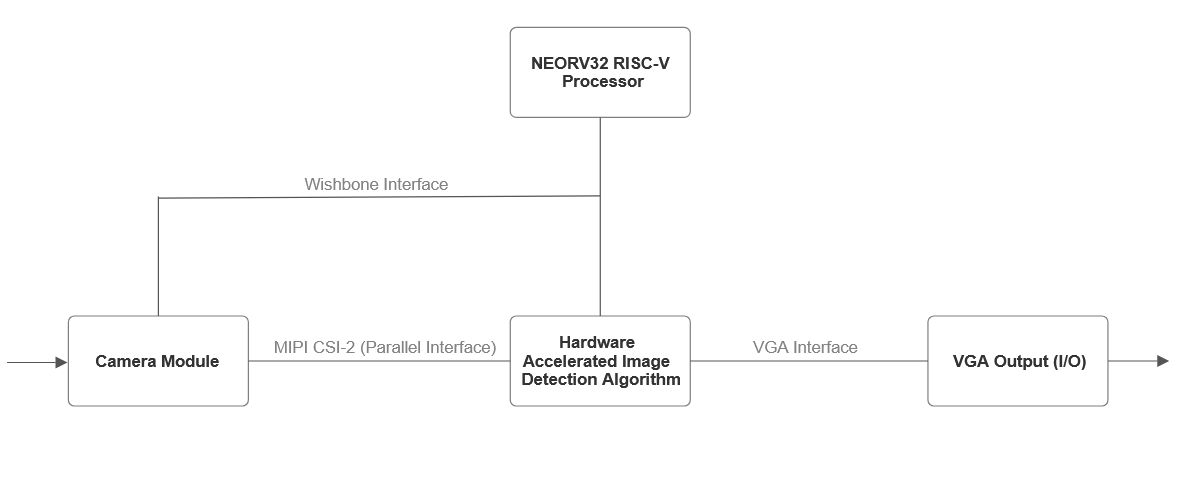
\includegraphics[width=1\textwidth]{Assets/Overview.png}
    \caption{Overview of proposed FPGA-based system.}
    \label{fig:overview}
\end{figure}

\subsection{Softcore Processor}
The NEORV32 RISC-V softcore processor has been selected due to it's highly documented ecosystem, and personal familiarity. 
This processor will be implemented as a SoC on the FPGA, and will be used to control the image detection algorithm and interface with the camera module.
A Wishbone b4 interface will be used to connect the processor to the FPGA.

\subsection{Image Detection Algorithm}
A convolutional neural network has been selected, such as in \cite{Gradient}, to be implemented on the FPGA for image detection.
Existing research has demonstrated that is not as resource intensive as other neural networks, and has noticeable advantages over traditional image detection algorithms.
Furthermore, image analysis is moving in the direction of deep learning algorithms for more complex image detection tasks, such as classification \cite{DCNN}.
By employing a CNN as the algorithm, the project will be able to demonstrate the capabilities of FPGA-based hardware acceleration for deep learning tasks and can be extended to a variety of domains.


\section{Performance Indicators}
The performance indicators of the system to establish the success of the project are provided in Table \ref{tab:performance} below.

\begin{center}
    \small
    \begin{longtable}{lp{0.6\linewidth}}
        \caption{Table of performance indicators.} \label{tab:performance}\\
        \toprule
        Indicator & Description \\
        \midrule
        \endfirsthead
        
        \caption{Performance indicators to assess the success of the project. (continued)} \\
        \toprule
        Indicator & Description \\
        \midrule
        \endhead
        
        \bottomrule
        \multicolumn{2}{r}{\textit{Continued on next page}} \\
        \endfoot
        
        \bottomrule
        \endlastfoot
        
        Algorithm accuracy      & The ability of the system to correctly detect features in an image. \\
        Scalability             & A measure of the limits of the system in terms of image size, image complexity and algorithm complexity \\
        Throughput              & Measured as the number of images processed per time unit \\
        Latency                 & The time delay between acquisition of image and output of results relative to the clock-speed of the Xilinx Artix 7 XC7A100T FPGA \\
        Resource Utilization    & The amount of FPGA resources used to implement the system specified by number of LUTs and BRAM required for implementation \\
    \end{longtable}
\end{center}

\section{Required Resources}
The hardware will be designed using both a Digilent Basys 3 development board for initial prototyping, before ideally being migrated to a Digilent Nexys A7-100T development board, to access more I/O and resources.
This prototyping step is done to demonstrate the implementation on severely resource constrained platforms, as per the scalability performance indicator. 
Both the selected boards have a VGA output, which can be used to display the processed image directly from the FPGA board. 
The specific camera module to be used has not yet been selected, however, a VGA OV7670 camera module which uses an I2C communication protocol is being considered for initial trials.
A VGA monitor will also be required to display the output of the processed image.

Benchmarking materials are dependent on the completed image detection algorithm selected, and cannot be provided at this time. 
Thus, the following resources are required for the project at this stage:

\begin{itemize}
    \item Xilinx Artix 7 XC7A100T FPGA
    \item Digilent Basys 3 FPGA Board
    \item Digilent Nexys A7 100T FPGA Board
    \item Camera Module
    \item VGA OV7670 Camera Module I2C
    \item VGA Monitor
    \item USB Power Supply
    \item VGA to VGA Cable / VGA to HDMI Cable
\end{itemize}


\chapter[Milestones]{Research Plan}

\label{Chap:Milestones}

\section{Milestones}
To track the development of the project, a set of milestones have been established with consideration of assessable dates. 
Table \ref{tab:milestones} below outlines the milestones for the work and what is required for each phase.
Emboldened text indicates an assessable milestone.


\begin{center}
    \small
    \begin{longtable}{p{0.25\linewidth}p{0.5\linewidth}p{0.15\linewidth}}
        \caption{Timeline of milestones.} \label{tab:milestones} \\
        \toprule
        Milestone & Description & Date \\
        \midrule
        \endfirsthead
        
        \caption{Timeline of milestones. (continued)} \\
        \toprule
        Milestone & Description & Date \\
        \midrule
        \endhead
        
        \bottomrule
        \multicolumn{3}{r}{\textit{Continued on next page}} \\
        \endfoot
        
        \bottomrule
        \endlastfoot
        
        \textbf{Project Proposal}	& Complete the project proposal and literature review.                                              & 21/3 \\
        Configure hardware			& Implement NEORV32 processor on FPGA, connect to external components through wishbone interface.   & 15/4 \\
        \textbf{Seminar}            & Present the current project status.                                                               & 6/5 \\
        Image detection algorithm   & Select and implement image detection algorithm in hardware.                                       & 12/8 \\
        VGA driver                  & Develop driver and interface to display processed image on VGA monitor.                           & 9/9 \\
        Benchmark                   & Benchmark system performance against related works.                                               & 4/10 \\
        \textbf{Demo}               & Demonstrate the complete project.                                                                 & 18/10 \\
        \textbf{Thesis}             & Document and write project results.                                                               & 4/11 \\
    \end{longtable}
\end{center}

\nopagebreak

The timeline was developed based on the expected time to completion for each task. A more detailed overview of the non-assessable tasks required for each milestone is provided in the following sections.

\subsection{Configure Hardware}
This task has been allocated three weeks of work, estimated at 20 hours of work. 
It entails the implementation of the NEORV32 processor on the FPGA, and the connection of the processor to the external components through the wishbone interface.

\subsection{Image Detection Algorithm}
This task has been allocated three months of work, estimated at 100 hours of work.
It requires the selection, implementation, and testing of the image detection algorithm in hardware.
Furthermore, it must additionally interface with the NEORV32 processor, and be able to be controlled by the processor.
As it is the core of the project, it has been allocated the most time.

\subsection{VGA Driver}
This task has been allocated four weeks of work, estimated at 30 hours of work.
The task requires the development of a driver and interface to display the processed image on a VGA monitor for the selected algorithm.
It is expected to be a relatively simple task, but has been allocated additional time for any unforeseen issues.

\subsection{Benchmark}
This task has been allocated four weeks of work, estimated at 30 hours of work.
It requires the benchmarking of the system performance against related works, and the documentation of the results.
The task is required to provide an assessment of the project's success against the performance indicators.


\section{Risk Assessment}
This project is conducted in the low-risk laboratory covered by general OHS laboratory rules, and in a home setting. 
There are no hazardous materials or dangerous equipment used in the project, and the risk of injury is negligible.
The only risk to the project is hardware failure or proprietary software issues, which can be mitigated by using open-source software and hardware, and regular backups of the project files.
Redundancies are also in place for hardware failure, as two FPGA developments boards are designated for use.

% HOW TO ADD ADDITIONAL CHAPTERS
% Step One: Add a new folder called "ChapterX" (X being the chapter number).
% Step Two: Within the folder add a new .tex file by clicking the "New File" button in the Overleaf Menu. Rename the file to a title of your choice.
% Step Three: Copy the Chapter 2 headline and "\input" command located above and insert it below Chapter 2.
% Step Four: Rename the headline to your specific chapter number, change the input command to include the name of the folder you created and the name of the file you created.
% Repeat this process for every chapter.

%CONCLUSION CHAPTER
% \chapter[Conclusion]{Conclusion}
\label{Chap:Conclusion}

This chapter summarizes the key findings and contributions of this thesis, discussing both the achievements and limitations of the hardware-based CNN implementation. Additionally, it outlines potential future work and recommendations for extending the design.

\section{Summary}

The research demonstrates the viability of hardware-accelerated convolution operations for resource-constrained embedded systems. Through the implementation and analysis of three distinct approaches to hardware convolution, this thesis has shown that effective trade-offs between parallelization and resource utilization are crucial for practical FPGA-based CNN acceleration.

The partially folded implementation emerged as the most effective solution, offering an optimal balance between resource utilization and performance. While the fully unrolled design theoretically offers maximum throughput, FPGA resource constraints, as discussed in Section \ref{sec:platforms}, made this approach impractical for real-world deployment. The fully folded implementation, despite its minimal resource usage, introduced significant control overhead that ultimately negated its resource advantages, aligning with the findings from previous research on hardware-based CNN implementations.

The integration with the NEORV32 RISC-V processor proved particularly significant, demonstrating a practical approach to hardware acceleration in SoC designs. As explored in the literature review, RISC-V's open-source nature and extensibility make it an ideal choice for embedded systems. The processor effectively manages data flow and control operations while offloading compute-intensive tasks to dedicated hardware accelerators, creating an efficient architecture for resource-constrained environments.

\section{Key Contributions}

This thesis contributes to the field of hardware-accelerated neural networks by developing configurable, generic hardware blocks for CNN implementation. This addresses the need for flexible, resource-efficient solutions in embedded systems. The successful integration with RISC-V demonstrates a practical approach to hardware acceleration, building upon existing research in FPGA-based CNN implementations.

The analysis of resource-performance trade-offs provides valuable insights for future FPGA-based CNN acceleration projects. The implementation of parallel MAC units with configurable folding factors offers a flexible solution that can be adapted to various resource constraints, addressing a key challenge identified in the literature review regarding the balance between parallelization and resource utilization.

\section{Limitations}

The research revealed several important limitations that warrant further investigation. Resource constraints fundamentally limit the maximum achievable parallelization, a challenge consistently noted in FPGA-based CNN implementations. As image and kernel sizes increase, timing constraints become increasingly problematic, necessitating more sophisticated approaches to maintain performance.

While the performance gap compared to GPU implementations is significant, this limitation stems from the inherent resource constraints of the target environment rather than the implementation approach. As discussed in Section \ref{sec:platforms}, GPUs benefit from thousands of CUDA cores and specialized architectures for parallel processing, advantages that cannot be replicated in resource-constrained FPGA environments.

The current implementation's lack of direct camera interface integration and the need for off-chip memory to store weights for large neural networks represent practical limitations that affect real-world deployment. These challenges align with those identified in previous research on embedded CNN implementations.

\section{Future Work}

Future research should focus on several key areas to address the identified limitations while maintaining the resource-efficient approach demonstrated in this thesis. Hardware optimizations could include the development of parallel adder trees or multi-cycle paths to address timing issues with larger kernels, building upon existing research in FPGA-based convolution implementations.

The RISC-V integration offers particularly promising avenues for future development. Custom instruction set extensions for CNN operations could further optimize performance, leveraging RISC-V's extensible nature as discussed in the literature review. The development of hardware-specific compiler optimizations and efficient memory-mapped interfaces could enhance the system's overall efficiency.

System integration represents another crucial area for future work. The integration of camera modules with real-time processing capabilities would enhance the practical applicability of the system. Development of efficient weight loading mechanisms and power management features would address current limitations in handling larger neural networks and improve system efficiency.

The generic nature of the developed hardware blocks provides a strong foundation for building complete CNN systems, while the RISC-V integration demonstrates a practical approach to hardware acceleration in embedded systems. Future work should focus on addressing the identified limitations while maintaining the resource-efficient approach demonstrated in this thesis.

In conclusion, this research highlights the potential of FPGA-based CNN acceleration for embedded systems, while acknowledging the inherent limitations of resource-constrained environments. The developed architecture, particularly the integration with RISC-V, provides a practical framework for future developments in hardware-accelerated machine learning applications. The findings contribute to the growing body of research on efficient hardware implementations of neural networks and offer valuable insights for future work in this field.




% ***************************************************
% Bibliography
%****************************************************
%CHOOSE YOUR BIB STYLE AND FILE.
%We have included the following two referencing styles for you to use in your thesis. You can add an alternate style if you prefer.

%Style: apalike = this is an (Author, Year) referencing style similar to APA
%Style: elsarticle-num = this is a numbered referencing style that will display the bibliography in citation order

%To use one of the styles provided ensure the % is removed from the start of the line, and the other option is commented out with a % at the start of the line. The style elsarticle-num is active by default.

\bibliographystyle{ieeetr}

\bibliography{./References/Bibliography}

%When you have finished your thesis we recommend that you manually fix any errors in your bibliography. 
%To do this, compile, copy the .bbl into a new .tex file and include this here after commenting out the other bibliography commands. Make corrections in that .tex file.

% ***************************************************
% Appendices
%**************************************************** 
%UNCOMMENT THIS SECTION IF YOU ARE USING APPENDICES.
%Simply adapt the same formatting used for other chapters.
% \appendix
% If you need appendix in your thesis then consider the following appendix file (you can add more if you need more) otherwise you should not consider it in your main thesis.
% % ***************************************************
% Appendix
% ***************************************************
\chapter{Appendix}

\section{Repository}
The repository for this project can be found at \url{https://github.com/jdw5/metr4911}.

\section{Device Information}
\label{app:device_information}

\subsection{CPU Device Specifications}
\begin{table}[h]
    \centering
    \begin{tabular}{|l|l|}
        \hline
        \textbf{Component} & \textbf{Specification} \\
        \hline
        Architecture & x86\_64 \\
        CPU Cores & 8 \\
        CPU Frequency & 3100 MHz \\
        System RAM & 90 GB Total \\
        GPU & N/A \\
        GPU Memory & N/A \\
        \hline
    \end{tabular}
    \caption{System Specifications for CPU Test Environment}
    \label{tab:cpu_specs}
\end{table}

\subsection{P100 Device Specifications}
\begin{table}[h]
    \centering
    \begin{tabular}{|l|l|}
        \hline
        \textbf{Component} & \textbf{Specification} \\
        \hline
        Architecture & x86\_64 \\
        CPU Cores & 20 (Physical) / 20 (Total) \\
        CPU Frequency & 3012.026 MHz \\
        System RAM & 251.55 GB Total \\
        GPU & Tesla P100-PCIE-16GB \\
        GPU Memory & 15.90 GB \\
        \hline
    \end{tabular}
    \caption{Device Specifications for P100 test environment}
    \label{tab:p100_specs}
\end{table}

\subsection{A100 Device Specifications}
\begin{table}[h]
    \centering
    \begin{tabular}{|l|l|}
        \hline
        \textbf{Component} & \textbf{Specification} \\
        \hline
        Architecture & x86\_64 \\
        CPU Cores & 8 \\
        CPU Frequency & 2894.562 MHz \\
        System RAM & 93.88 GB Total \\
        GPU & NVIDIA A100-PCIE-40GB \\
        GPU Memory & 39.39 GB \\
        \hline
    \end{tabular}
    \caption{Device Specifications for A100 test environment}
    \label{tab:a100_specs}
\end{table}


\section{Convolution Results}

\subsection{CPU}
\begin{table}[h]
    \centering
    \begin{tabular}{|c|c|}
        \hline
        \textbf{Test Number} & \textbf{Execution Time (ns)} \\
        \hline
        1 & 213342 \\
        2 & 223891 \\
        3 & 229782 \\
        4 & 249048 \\
        5 & 252755 \\
        \hline
    \end{tabular}
    \caption{CPU Convolution Execution Times}
    \label{tab:cpu_conv_times}
\end{table}

\textbf{Test Configuration:}
\begin{itemize}
    \item Input Size: 8 x 8 x 1
    \item Kernel Size: 2 x 2 x 1 x 10
    \item Output Feature Size: 7 x 7 x 10
    \item Resolution: 8-bit
    \item Stride Steps: 1
    \item Zero Padding: 0
\end{itemize}

\subsection{P100}
\begin{table}[h]
    \centering
    \begin{tabular}{|c|c|}
        \hline
        \textbf{Test Number} & \textbf{Execution Time (ns)} \\
        \hline
        1 & 1010.27 \\
        3 & 1016.85 \\
        3 & 1020.45 \\
        4 & 1056.34 \\
        5 & 1120.34 \\
        \hline
    \end{tabular}
    \caption{A100 Convolution Execution Times}
    \label{tab:a100_conv_times}
\end{table}

% You might want to add these statistics
\textbf{Test Configuration:}
\begin{itemize}
    \item Input Size: 8 x 8 x 1
    \item Kernel Size: 2 x 2 x 1 x 10
    \item Output Feature Size: 7 x 7 x 10
    \item Resolution: 8-bit
    \item Stride Steps: 1
    \item Zero Padding: 0
\end{itemize}

\subsection{A100}
\begin{table}[h]
    \centering
    \begin{tabular}{|c|c|}
        \hline
        \textbf{Test Number} & \textbf{Execution Time (ns)} \\
        \hline
        1 & 608.35 \\
        2 & 608.73 \\
        3 & 610.98 \\
        4 & 612.70 \\
        5 & 613.58 \\
        \hline
    \end{tabular}
    \caption{P100 Convolution Execution Times}
    \label{tab:p100_conv_times}
\end{table}

\textbf{Test Configuration:}
\begin{itemize}
    \item Input Size: 8 x 8 x 1
    \item Kernel Size: 2 x 2 x 1 x 10
    \item Output Feature Size: 7 x 7 x 10
    \item Resolution: 8-bit
    \item Stride Steps: 1
    \item Zero Padding: 0
\end{itemize}

\newpage
\section{HDL Type Primitive}
\label{app:hdl_type_primitive}

A custom hardware type primitive was created for this project. 
It represents a feature with a height, width and depth to simplify the hardware design.

\begin{lstlisting}[language=VHDL]
type feature_t is array(natural range <>, natural range <>, natural range <>) of signed;
\end{lstlisting}

\section{Schematics}
The below pages are the hardware schematics for the project.
These are provided at high resolution to allow for detailed inspection.
The first page provided is the accelerator component, which describes the linking of the generic layers.
The second schematic is the accelerator connected to block RAMs to pass the weights and bias signals. It wraps the accelerator in a block RAM interface.
The third schematic is the system on chip, which receives the input image from the NeoRV32 softcore processor. It implements the previous schematic as an IP core.

\newpage
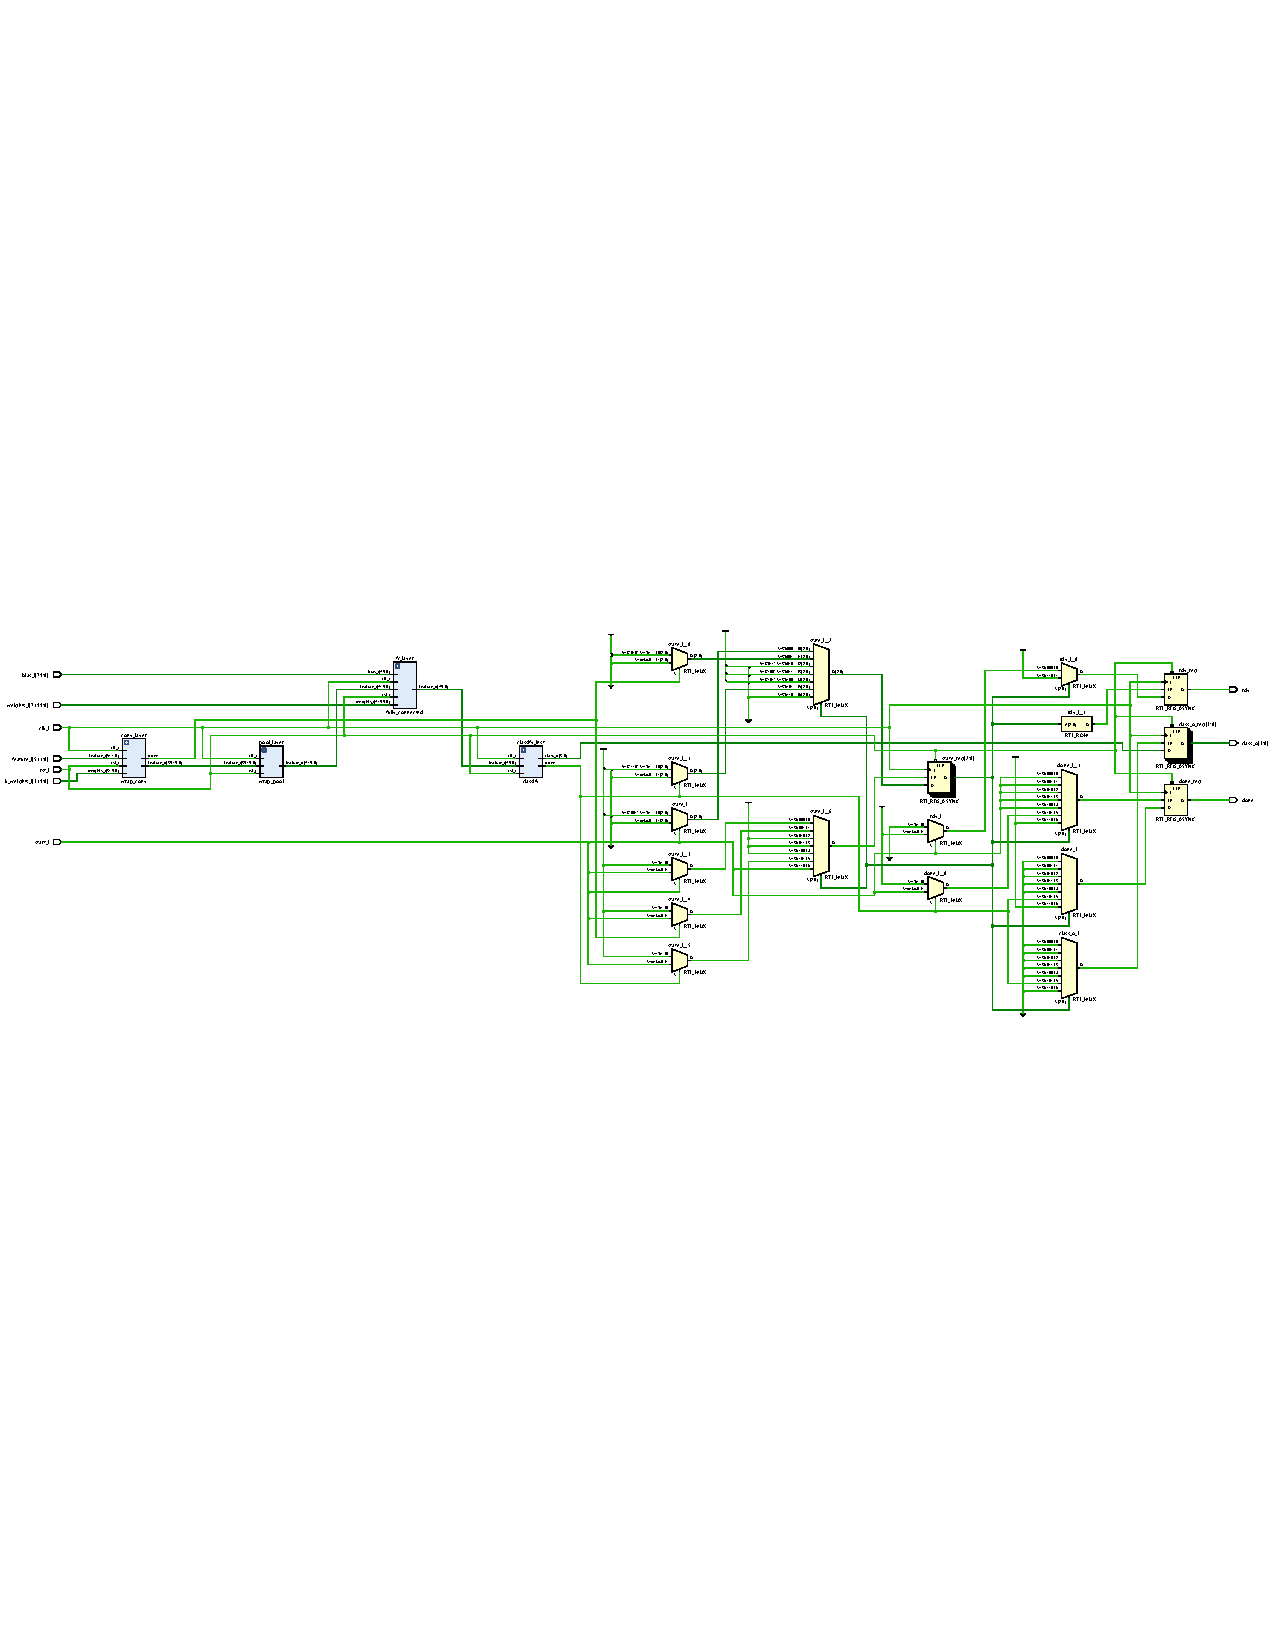
\includepdf[pages=-]{Figs/accelerator.pdf}

\newpage
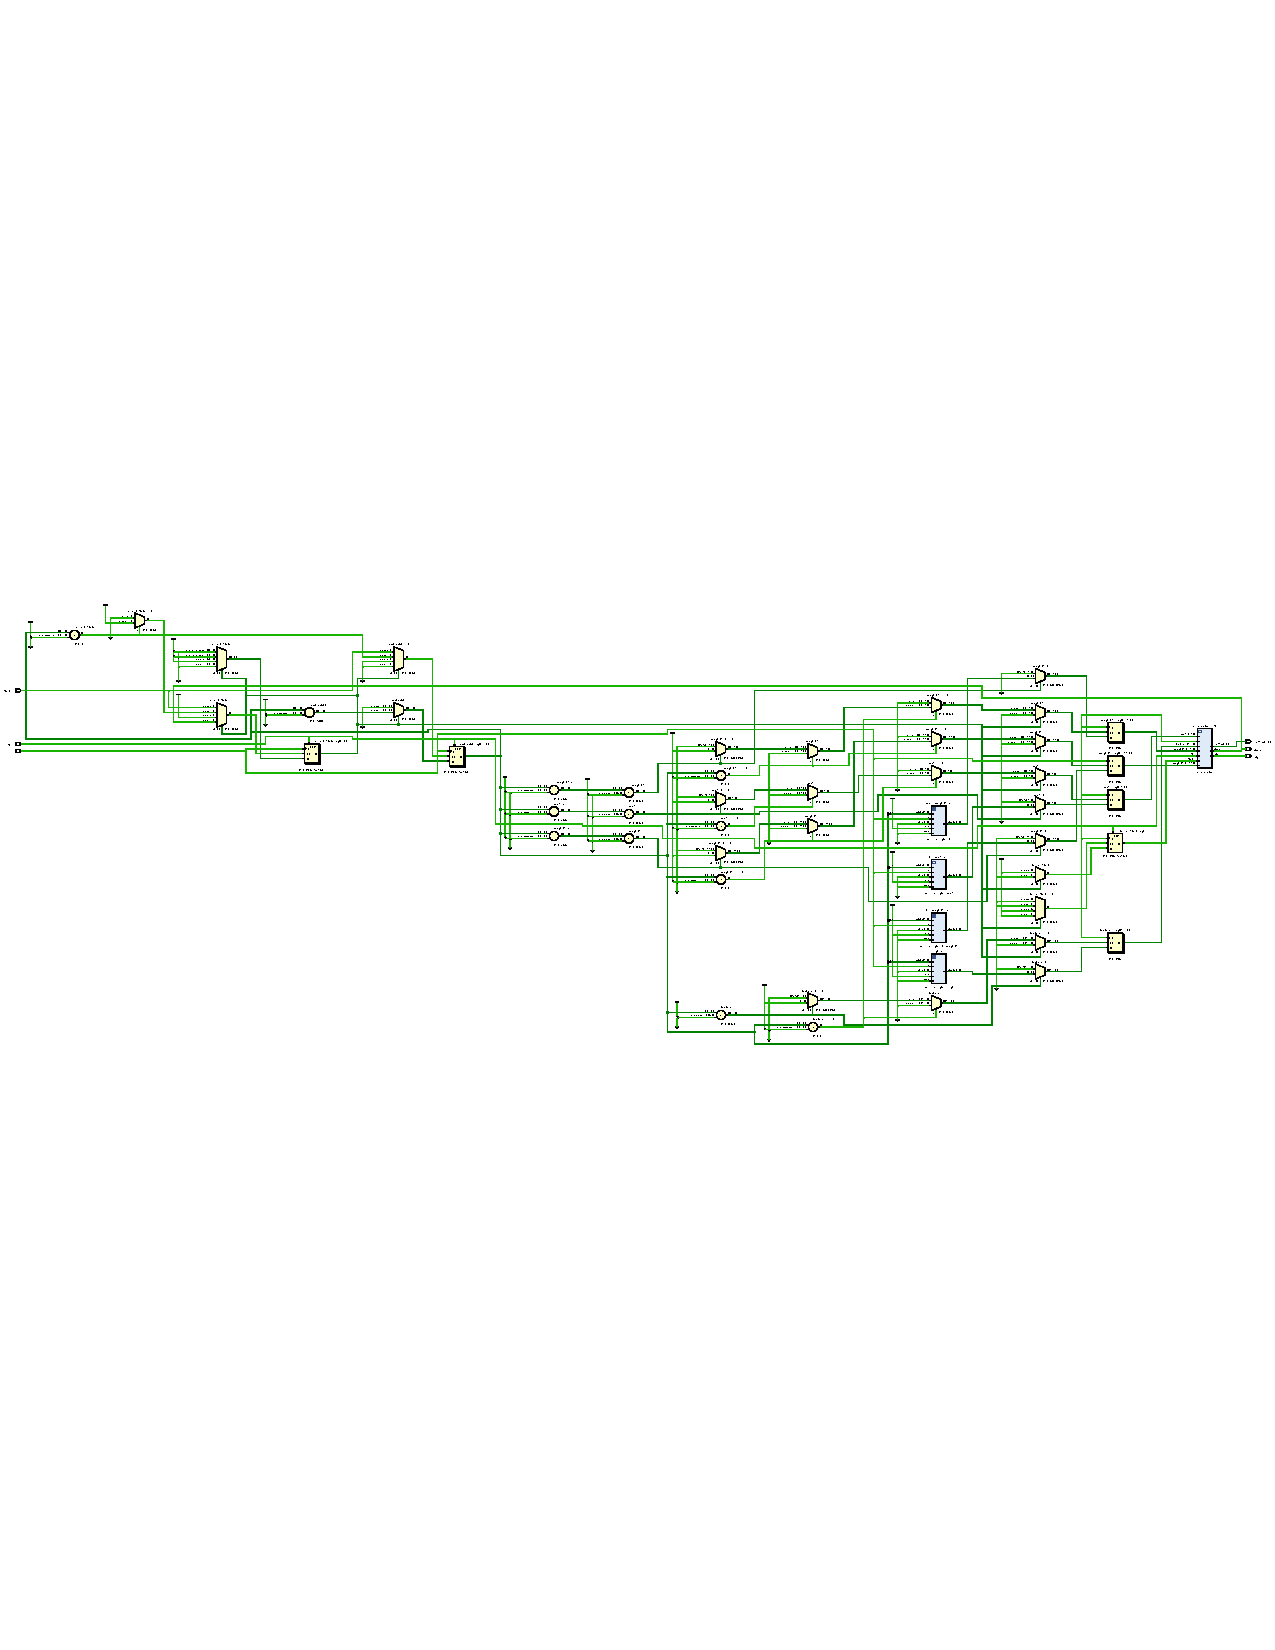
\includepdf[pages=-]{Figs/mem_accelerator.pdf}

\newpage
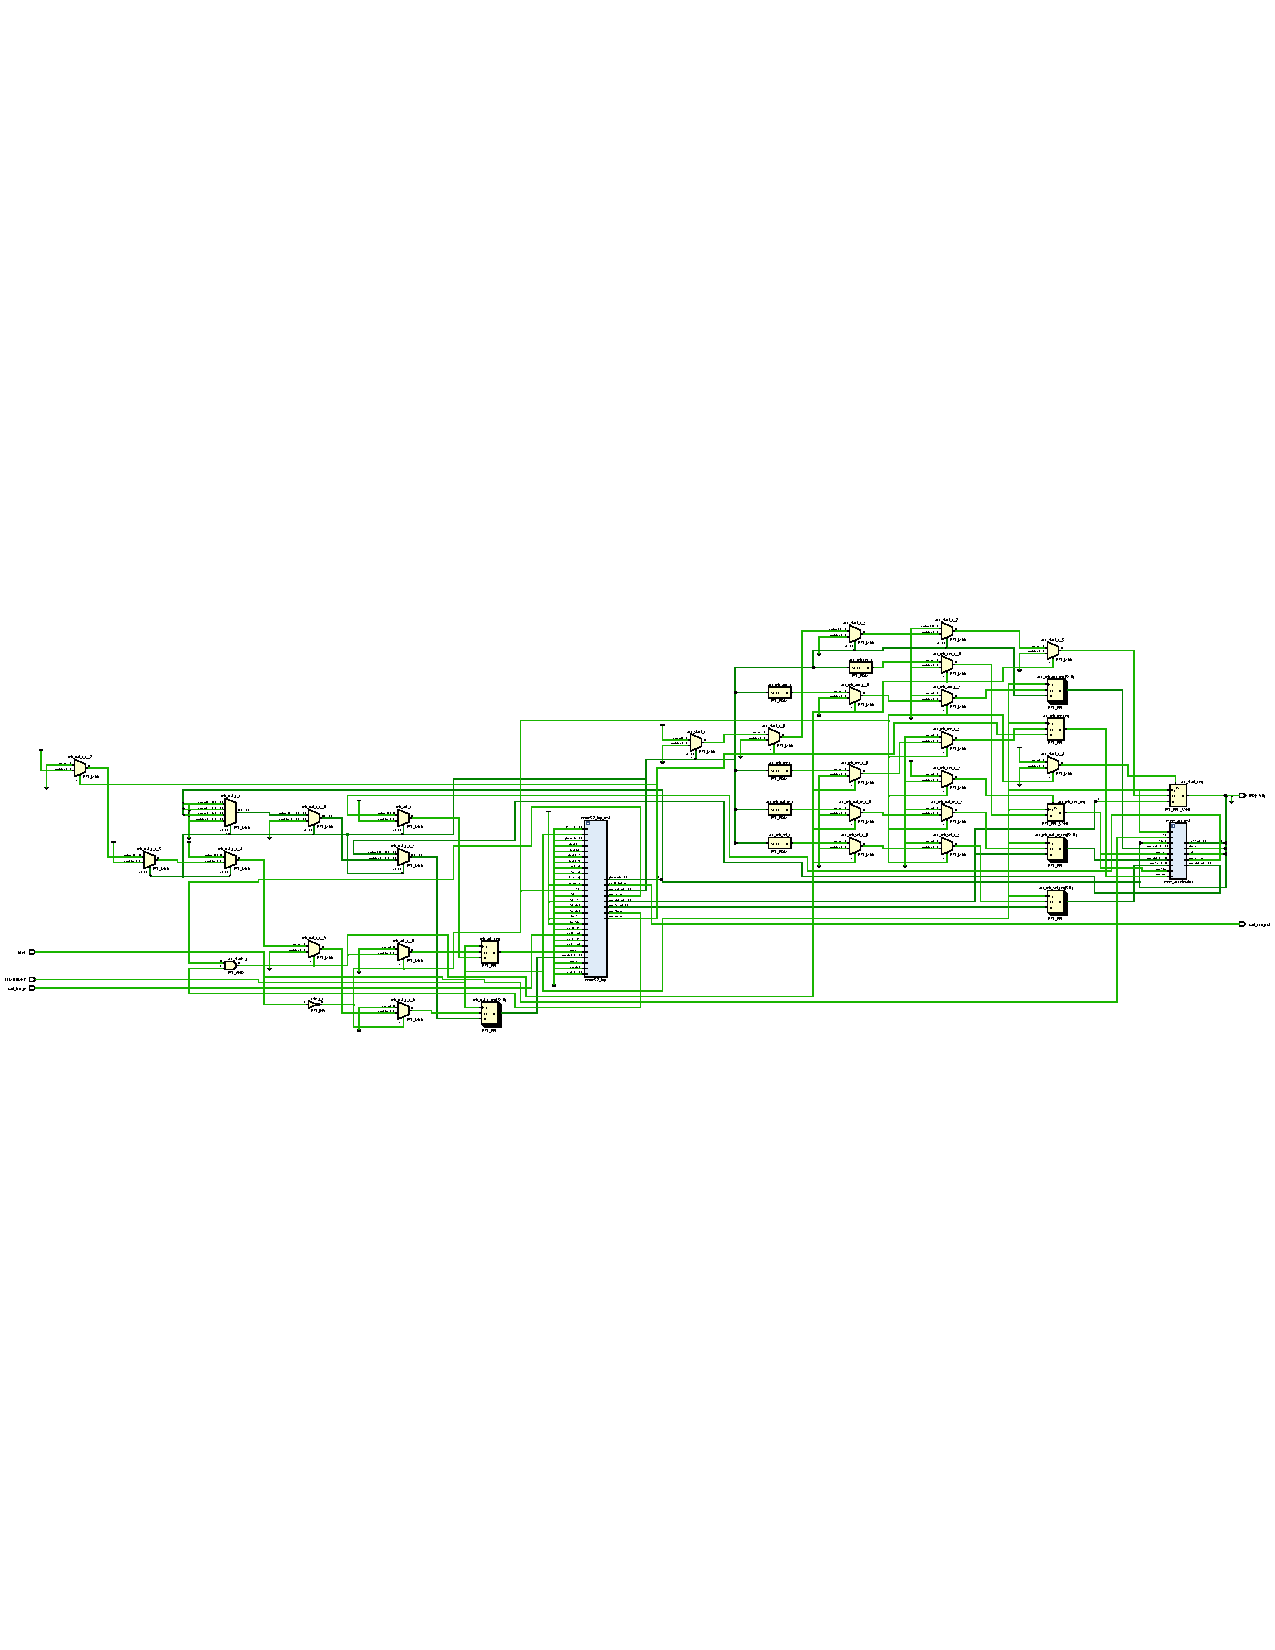
\includepdf[pages=-]{Figs/riscv-ml-core.pdf}


% ***************************************************
% Examples
%**************************************************** 
% The following files are only for examples and you should not include them in your final thesis.
% \include{./Examples/ExampleOfCitations}
% \include{./Examples/ExampleOfCode}
% \include{./Examples/ExampleOfEquations}
% \include{./Examples/ExampleOfFigures}
% \include{./Examples/ExampleOfFlowCharts}
% \include{./Examples/ExampleOfTables}


% ***************************************************
% Back Matter
%**************************************************** 
% COMMENT OUT IF YOU DO NOT WISH TO INCLUDE BACK MATTER.
% \input{./PreliminaryAndBackPages/Back.tex}

\end{document}
